\documentclass[11pt,a4paper]{report}

\usepackage[french]{babel}
\usepackage[utf8]{inputenc}
\usepackage[T1]{fontenc}
\usepackage{lmodern}
\usepackage{geometry}
\usepackage{graphicx}
\usepackage{float}
\usepackage{booktabs}
\usepackage{tabularx}
\usepackage{array}
\usepackage{longtable}
\usepackage{xcolor}
\usepackage{tikz}
\usetikzlibrary{arrows.meta,positioning,shapes.geometric,fit,calc}
\usepackage{listings}
\usepackage{hyperref}
\usepackage{fancyhdr}
\usepackage{titlesec}
\usepackage{enumitem}
\usepackage{caption}
\usepackage{subcaption}
\usepackage{amsmath}
\usepackage{pgfplots}
\pgfplotsset{compat=1.18}
\usepackage{lastpage}

\geometry{margin=2cm,headheight=14pt}
\definecolor{navy}{HTML}{183B56}
\definecolor{blue}{HTML}{2F75B5}
\definecolor{orange}{HTML}{F39C12}
\definecolor{green}{HTML}{2E8B57}
\definecolor{lightgray}{HTML}{F2F4F7}
\definecolor{gold}{HTML}{D4A72C}
\definecolor{red}{HTML}{C0392B}

\hypersetup{
  colorlinks=true,
  linkcolor=navy,
  urlcolor=blue,
  pdftitle={Entrepôt de données temps réel avec PostgreSQL, Kafka, Spark, HDFS, Hive et Streamlit},
  pdfauthor={Bilal Ziyane}
}

\pagestyle{fancy}
\fancyhf{}
\lhead{\textcolor{navy}{Projet DataOps -- Entrepôt temps réel}}
\rhead{\textcolor{navy}{Bilal Ziyane}}
\cfoot{\thepage/\pageref{LastPage}}
\renewcommand{\headrulewidth}{0.4pt}
\renewcommand{\chaptername}{Partie}

\titleformat{\chapter}[display]
  {\normalfont\Large\bfseries\color{navy}}
  {\chaptertitlename\ \thechapter}{15pt}{\huge}
\titlespacing*{\chapter}{0pt}{-20pt}{30pt}

\lstset{
  basicstyle=\ttfamily\small,
  keywordstyle=\color{blue},
  commentstyle=\color{green},
  stringstyle=\color{orange},
  frame=single,
  rulecolor=\color{gray},
  backgroundcolor=\color{lightgray},
  breaklines=true,
  columns=fullflexible,
  showstringspaces=false,
  captionpos=b
}

\newcolumntype{Y}{>{\raggedright\arraybackslash}X}
\newcommand{\tabletag}[1]{\colorbox{lightgray}{\texttt{\small #1}}}
\newcommand{\good}[1]{\textcolor{green}{\textbf{#1}}}
\newcommand{\warn}[1]{\textcolor{orange}{\textbf{#1}}}
\newcommand{\bad}[1]{\textcolor{red}{\textbf{#1}}}

\begin{document}

\hypersetup{pageanchor=false}

\begin{titlepage}
\begin{tikzpicture}[remember picture,overlay]
  \fill[navy] (current page.north west) rectangle ([yshift=-8.5cm]current page.north east);
  \fill[orange] ([yshift=-8.5cm]current page.north west) rectangle ([yshift=-8.72cm]current page.north east);
\end{tikzpicture}
\vspace*{2.0cm}
\begin{center}
{\color{white}\Large PROJET DATAOPS}\\[0.5cm]
{\color{white}\fontsize{28}{34}\selectfont\bfseries Entrepôt de données temps réel}\\[0.35cm]
{\color{white}\large PostgreSQL, Kafka, Spark, HDFS, Hive et Streamlit}\\[1.8cm]
\begin{tikzpicture}
\node[draw=navy,rounded corners=5pt,fill=white,minimum width=13cm,minimum height=2.2cm,
      text width=12cm,align=center] {
  \Large Pipeline batch et streaming\\
  \normalsize De l'ingestion aux requêtes analytiques HiveQL
};
\end{tikzpicture}
\vfill
\begin{tabular}{ll}
\textbf{Réalisé par} & Bilal Ziyane\\
\textbf{Formation} & Master Data \& IA\\
\textbf{Date} & Novembre 2026\\
\textbf{Environnement} & Podman -- Fedora Linux -- Spark 4.0.1 -- Hive 4.0.1
\end{tabular}
\end{center}
\end{titlepage}

\hypersetup{pageanchor=false}
\pagenumbering{roman}
\chapter*{Résumé exécutif}
\addcontentsline{toc}{chapter}{Résumé exécutif}

Ce projet réalise un entrepôt de données transactionnel combinant ingestion
batch et temps réel. PostgreSQL constitue la source opérationnelle ;
Apache Spark transforme les données ; HDFS les organise dans des couches
Bronze, Silver, Gold et Quarantine ; Apache Kafka transporte les événements
temps réel ; Apache Hive publie les tables externes par un Metastore ; enfin,
Streamlit offre un tableau de bord interactif.

PostgreSQL remplace volontairement SQL Server, demandé par le professeur dans
le schéma de référence. Cette substitution est documentée et prend en charge
un volume opérationnel reproduisible ainsi que les métriques Gold.

L'exécution observée utilise un NameNode, une DataNode HDFS et un worker Spark.
Les contrôles ont confirmé
\textbf{149\,823 transactions sources}, \textbf{720 lignes Gold},
\textbf{5 tables Hive externes}, un NameNode actif, une DataNode vivante,
un worker Spark actif et HDFS hors \em{safe mode}.

\textbf{Mots-clés :} DataOps, PostgreSQL, Apache Kafka, Apache Spark,
HDFS, Apache Hive, HiveQL, Streamlit, architecture en médaillon, temps réel,
données transactionnelles.

\tableofcontents
\listoffigures
\listoftables
\clearpage
\hypersetup{pageanchor=true}
\pagenumbering{arabic}

\chapter{Introduction}

\section{Contexte et problème métier}
Le cas d'étude concerne une plateforme de suivi des transactions financières.
Une base opérationnelle doit enregistrer rapidement les paiements, tandis que
les équipes d'analyse doivent retrouver l'historique, les tendances,
les pertes, les statuts et les risques. Interroger directement la base
opérationnelle pour produire ces agrégations mélange les responsabilités :
elle concentre les écritures transactionnelles et ne garantit pas une vue
analytique stable ou historique.

L'entrepôt construit dans ce projet sépare donc l'opérationnel de l'analyse.
La base PostgreSQL reste la source durable. Spark lit les événements,
les valide, les déduplique et les transforme. HDFS conserve les résultats
dans des couches explicites. Hive met des noms de tables sur ces fichiers
Parquet. Streamlit montre les indicateurs issus des données Gold.

\section{Objectifs}
\begin{enumerate}[leftmargin=*]
\item Implémenter le pipeline décrit par l'architecture de référence.
\item Remplacer SQL Server par PostgreSQL selon le choix validé.
\item Ingérer des données par lots à partir de PostgreSQL.
\item Introduire Kafka et Spark Structured Streaming.
\item Structurer les données en couches Bronze, Silver, Gold et Quarantine.
\item Publier les données HDFS dans le catalogue Apache Hive.
\item Fournir un tableau de bord Streamlit.
\item Documenter, automatiser et tester les opérations.
\end{enumerate}

\section{Cahier des charges respecté}
Le schéma fourni fixait principalement les briques suivantes : source
relationnelle, Spark comme moteur d'intégration et d'analyse, HDFS comme
stockage distribué, architecture Bronze/Silver/Gold, Metastore Hive et
différents profils utilisateurs. La réalisation respecte ces principes
avec les adaptations suivantes :
\begin{itemize}
\item PostgreSQL est utilisé à la place de SQL Server.
\item Kafka est ajouté comme canal temps réel.
\item Streamlit fournit le tableau de bord de démonstration.
\item YARN et des DataNodes supplémentaires sont disponibles dans le profil \texttt{full}.
\item Hive est démarré avec son Metastore et HiveServer2 pour exposer les tables HDFS.
\item Le Metastore Hive utilise Derby persistant ; PostgreSQL reste la source opérationnelle et la cible Gold.
\end{itemize}

\section{Périmètre du rapport}
Ce rapport décrit l'architecture, les données, l'implémentation, les validations,
les résultats observés, les limites techniques et les procédures de démonstration.
Le déploiement présenté est un environnement de cours : il utilise une DataNode
et ne fournit pas de haute disponibilité ni de réplication distribuée.

\chapter{Architecture globale}

\section{Schéma de référence}
La figure~\ref{fig:reference} reproduit l'image fournie avec le sujet.
Elle guide l'organisation des couches et des responsabilités.

\begin{figure}[H]
\centering
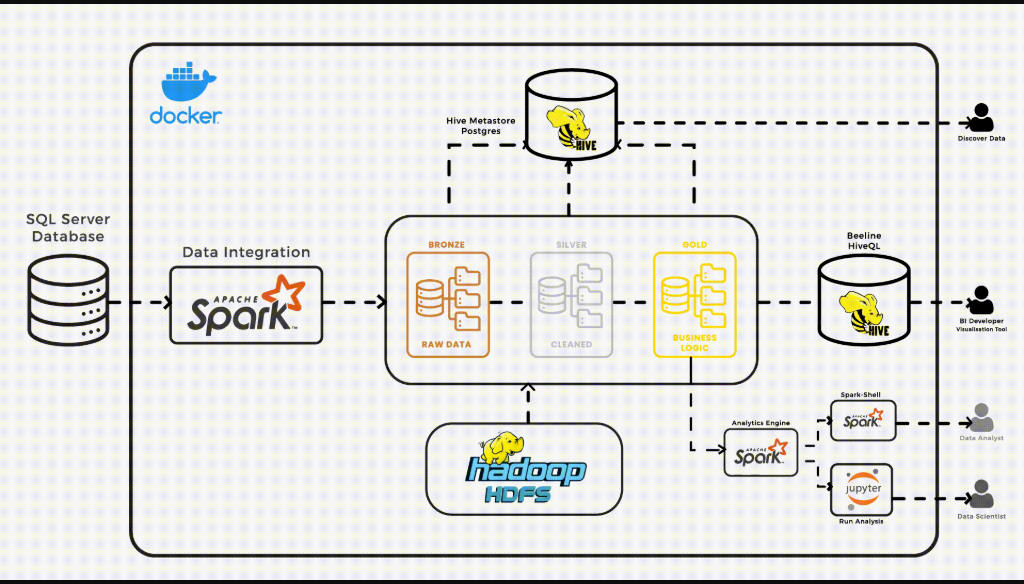
\includegraphics[width=.92\textwidth]{figures/reference_architecture_cropped.png}
\caption{Schéma de référence fourni avec le projet.}
\label{fig:reference}
\end{figure}

\section{Architecture physique implémentée}
\begin{figure}[H]
\centering
\resizebox{\textwidth}{!}{%
\begin{tikzpicture}[node distance=8mm and 9mm,>=Stealth,
  box/.style={draw,rounded corners=3pt,minimum height=12mm,text width=27mm,
              align=center,fill=lightgray,font=\small},
  core/.style={box,fill=blue!12},
  data/.style={box,fill=gold!18},
  biz/.style={box,fill=green!12},
  optional/.style={box,fill=orange!12}]
\node[core] (pg) {PostgreSQL\\Source};
\node[core,right=of pg] (sparkb) {Spark Batch\\JDBC};
\node[data,right=of sparkb] (bronze) {Bronze\\Parquet};
\node[data,right=of bronze] (silver) {Silver\\Dédup.};
\node[data,right=of silver] (gold) {Gold\\Métriques};
\draw[->,thick] (pg) -- (sparkb);
\draw[->,thick] (sparkb) -- (bronze);
\draw[->,thick] (bronze) -- (silver);
\draw[->,thick] (silver) -- (gold);
\node[core,below=12mm of pg] (producer) {Producteur\\Python};
\node[core,right=of producer] (kafka) {Kafka};
\node[core,right=of kafka] (sparks) {Spark\\Structured Streaming};
\node[biz,right=of sparks] (enrich) {Enrichissement};
\node[data,right=of enrich] (enriched) {Gold enrichi\\HDFS/Parquet};
\draw[->,thick] (kafka) -- (sparks);
\draw[->,thick] (producer) -- (kafka);
\draw[->,thick] (sparks) -- (enrich);
\draw[->,thick] (enrich) -- (enriched);
\draw[->,thick] (producer.north) -- (pg.south);
\node[optional,below=12mm of silver] (hive) {Hive Metastore\\+ HiveServer2};
\node[optional,right=of hive] (streamlit) {Streamlit\\PostgreSQL Gold};
\node[optional,left=of hive] (hdfs) {HDFS NameNode\\+ 1 DataNode};
\draw[<->,thick] (hdfs) -- (hive);
\draw[->,thick] (gold.south) |- (hdfs.north);
\draw[->,thick] (enriched.south) |- (hdfs.east);
\end{tikzpicture}
}
\caption{Architecture physique et logique du projet.}
\label{fig:archphysical}
\end{figure}

\section{Flux batch}
Le chargement batch suit un chemin déterministe : extraction incrémentale depuis
PostgreSQL, ajout dans HDFS Bronze, lecture globale des données Bronze, nettoyage,
déduplication et publication Silver/Gold. Un watermark basé sur la date de
création et l'identifiant de transaction évite de relire inutilement les lignes
déjà traitées.

\section{Flux temps réel}
Le producteur insère chaque nouvelle transaction dans PostgreSQL et publie aussi
son JSON sur le topic \texttt{transactions\_topic}. Spark Structured Streaming
lit ce topic, ajoute les informations clients et moyens de paiement, calcule
les frais, la latence, le niveau de risque et la catégorie, puis écrit vers
\texttt{enriched\_transactions\_topic} et HDFS Parquet.

\chapter{Modèle de données et qualité}

\section{Schéma PostgreSQL}
\begin{figure}[H]
\centering
\begin{tikzpicture}[node distance=20mm,
  ent/.style={draw,rounded corners=2pt,fill=lightgray,minimum width=55mm,
              text width=50mm,align=left,font=\scriptsize},
  gold/.style={draw,rounded corners=2pt,fill=gold!15,minimum width=55mm,
               text width=50mm,align=left,font=\scriptsize}]
\node[ent] (trans) {\textbf{public.transactions}\\
\_\_ transaction\_id UUID PK\\
customer\_id, payment\_method\_id\\
country\_id, merchant\_id\\
transaction\_type, amount, currency\\
status, device\_type\\
producer\_timestamp\_ms, reference\\
created\_at};
\node[gold,right=of trans] (gold) {\textbf{gold.daily\_transaction\_metrics}\\
transaction\_date\\
currency, status, transaction\_type\\
transaction\_count\\
gross\_amount, average\_amount};
\draw[->,thick] (trans) -- node[above]{\scriptsize agrégation Spark} (gold);
\end{tikzpicture}
\caption{Modèle relationnel simplifié.}
\label{fig:pgmodel}
\end{figure}

\section{Données de démonstration}
Le script d'initialisation crée cinq transactions déterministes permettant
de vérifier immédiatement une source reproductible. Le producteur ajoute
ensuite des transactions aléatoires réalistes avec des identifiants,
montants, devises, statuts et types cohérents.

La devise est contrôlée selon le pays : US/USD, UK/GBP, DE et FR/EUR,
IN/INR, CA/CAD et AU/AUD. Les dimensions clients et moyens de paiement
sont chargées depuis les fichiers CSV montés dans Spark.

\section{Règles de qualité}
\begin{table}[H]
\centering
\begin{tabularx}{\textwidth}{l Y Y}
\toprule
\textbf{Règle} & \textbf{Motif de rejet} & \textbf{Traitement}\\
\midrule
Champs obligatoires & missing\_required\_field & Quarantine\\
Montant négatif & negative\_amount & Quarantine\\
Statut inconnu & invalid\_status & Quarantine\\
Type inconnu & invalid\_transaction\_type & Quarantine\\
Horodatage invalide & invalid\_timestamp & Quarantine\\
Transaction identique & Déduplication & Dernière ligne conservée\\
\bottomrule
\end{tabularx}
\caption{Règles appliquées avant publication Silver.}
\end{table}

\section{Architecture en médaillon}
\begin{figure}[H]
\centering
\begin{tikzpicture}[node distance=12mm,
bronze/.style={draw,rounded corners=4pt,fill=orange!25,minimum width=42mm,minimum height=24mm,align=center},
silver/.style={draw,rounded corners=4pt,fill=gray!18,minimum width=42mm,minimum height=24mm,align=center},
gold/.style={draw,rounded corners=4pt,fill=gold!30,minimum width=42mm,minimum height=24mm,align=center}]
\node[bronze] (b) {\textbf{BRONZE}\\Données brutes\\Append\\Parquet};
\node[silver,right=of b] (s) {\textbf{SILVER}\\Déduplication\\Validation\\Snapshot};
\node[gold,right=of s] (g) {\textbf{GOLD}\\Métriques\\Agrégations\\PostgreSQL/Hive};
\draw[->,very thick] (b) -- (s);
\draw[->,very thick] (s) -- (g);
\end{tikzpicture}
\caption{Organisation des couches en médaillon.}
\label{fig:medallion}
\end{figure}

\chapter{Implémentation batch}

\section{Lecture incrémentale PostgreSQL}
Le job Spark lit PostgreSQL via un pilote JDBC. Au premier lancement, le
watermark HDFS n'existe pas et toutes les lignes sont chargées. Les lancements
suivants filtrent les lignes à partir de la date de création et de l'identifiant
de transaction.
Le watermark n'est avancé qu'après l'écriture réussie de Bronze.

\begin{lstlisting}[language=SQL,caption={Lecture incrémentale JDBC dans Spark}]
(SELECT * FROM public.transactions
 WHERE (created_at, transaction_id) >
       (TIMESTAMPTZ '2026-11-20 01:00:00+00',
        '550e8400-e29b-41d4-a716-446655440000'::uuid)
) AS incremental_transactions
\end{lstlisting}

\section{Écriture Bronze}
Les nouvelles lignes sont ajoutées en Parquet et partitionnées par date.
La base opérationnelle reste séparée du stockage analytique.

\section{Construction Silver}
Une fenêtre Spark partitionnée par \texttt{transaction\_id} ordonne les
doublons selon la date de création et l'horodatage producteur. Une seule
occurrence est conservée. Les lignes invalides sont extraites dans
\texttt{/warehouse/silver/quarantine}.

\section{Construction Gold}
Les métriques Gold agrègent les transactions par date, devise, statut et type.
Elles contiennent :
\begin{itemize}
\item \texttt{transaction\_count}
\item \texttt{gross\_amount}
\item \texttt{average\_amount}
\end{itemize}

Le résultat est écrit dans HDFS et dans la table Gold de PostgreSQL.

\section{Résultats du chargement batch}
Une exécution a chargé des données dans toutes les zones en médaillon. Les
validations ont montré \textbf{149\,823 transactions sources} et
\textbf{720 lignes Gold}. La zone quarantine contient un fichier Parquet
dont la taille est mesurable dans HDFS.

\chapter{Implémentation temps réel}

\section{Producteur}
Le producteur Python génère des transactions avec UUID, pays, type, montant,
devise, statut, marchand, appareil et horodatage. Il effectue deux actions :
\begin{enumerate}
\item insertion durable dans PostgreSQL ;
\item publication dans \texttt{transactions\_topic}.
\end{enumerate}

Le paramètre \texttt{acks=all} demande l'accusé Kafka avant confirmation.

\section{Spark Structured Streaming}
Spark lit Kafka depuis \texttt{broker:29092}, avec le mode
\texttt{earliest} et un intervalle micro-batch configurable.
Les données sont jointes avec les dimensions clients et moyens de paiement
chargées depuis les CSV.

\begin{lstlisting}[language=Python,caption={Source Kafka du pipeline Streaming}]
source = (
    spark.readStream
    .format("kafka")
    .option("kafka.bootstrap.servers", "broker:29092")
    .option("subscribe", "transactions_topic")
    .option("startingOffsets", "earliest")
    .load()
)
\end{lstlisting}

\section{Enrichissements métier}
\begin{table}[H]
\centering
\begin{tabularx}{\textwidth}{l Y}
\toprule
\textbf{Attribut calculé} & \textbf{Rôle}\\
\midrule
processing\_fee\_amount & Montant = amount $\times$ fee percentage\\
is\_high\_value & Montant supérieur ou égal à 100\\
is\_premium\_customer & Client premium ou gold\\
risk\_score & LOW, MEDIUM ou HIGH\\
transaction\_category & revenue, loss ou neutral\\
e2e\_latency\_ms & Timestamp Kafka moins horodatage producteur\\
\bottomrule
\end{tabularx}
\caption{Transformations du flux temps réel.}
\end{table}

\section{Sinks Kafka et HDFS}
Le même DataFrame enrichi est publié sur
\texttt{enriched\_transactions\_topic} puis écrit en Parquet dans
\texttt{/warehouse/gold/enriched\_transactions}. Les checkpoints
Spark sont conservés dans HDFS afin de reprendre après redémarrage.

\begin{figure}[H]
\centering
\begin{tikzpicture}[node distance=7mm and 6mm,>=Stealth,
  nodebox/.style={draw,rounded corners=3pt,fill=lightgray,text width=24mm,
                  minimum height=13mm,align=center,font=\scriptsize}]
\node[nodebox,fill=blue!10] (producer) {Producteur\\Python};
\node[nodebox,right=of producer] (pg) {PostgreSQL};
\node[nodebox,right=of pg] (in) {Kafka\\transactions};
\node[nodebox,right=of in] (spark) {Spark\\Streaming};
\node[nodebox,right=of spark,fill=gold!20] (out) {Kafka enrichi};
\node[nodebox,below=10mm of out,fill=green!12] (hdfs) {HDFS\\Enriched Gold};
\draw[->,thick] (producer) -- (pg);
\draw[->,thick] (producer) -- (in);
\draw[->,thick] (pg) -- (in);
\draw[->,thick] (in) -- (spark);
\draw[->,thick] (spark) -- (out);
\draw[->,thick] (spark) |- (hdfs);
\end{tikzpicture}
\caption{Chemin du flux temps réel.}
\label{fig:streaming}
\end{figure}

\chapter{Stockage HDFS}

\section{NameNode et DataNode}
HDFS utilise un NameNode et une DataNode active. Le facteur de réplication
est fixé à 1 dans le déploiement mono-nœud présenté. Les paramètres de safe
mode permettent au cluster de devenir disponible après son démarrage.

\begin{figure}[H]
\centering
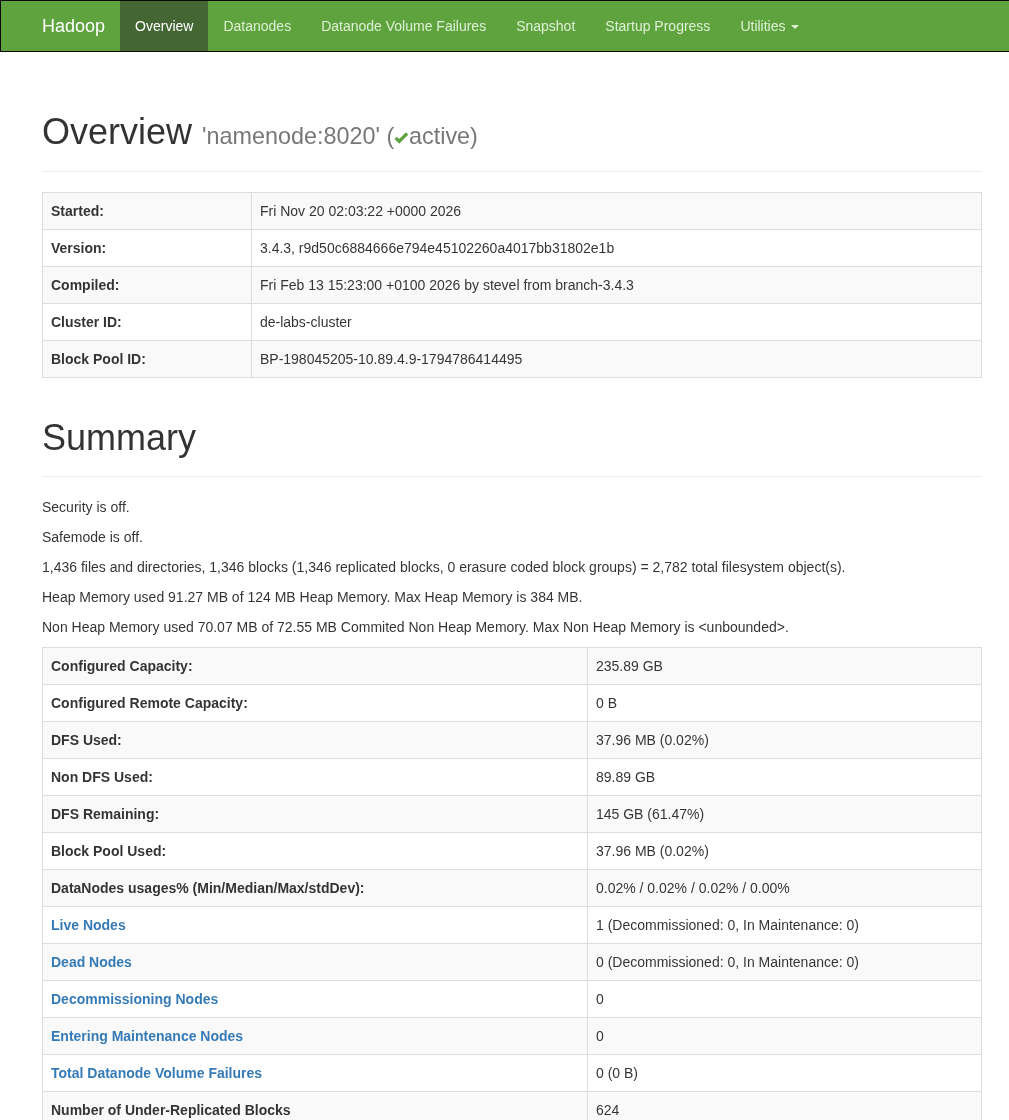
\includegraphics[width=.92\textwidth,height=.70\textheight,keepaspectratio]{figures/hdfs_namenode_summary.png}
\caption{Interface HDFS NameNode finale : safe mode OFF et une DataNode vivante.}
\label{fig:hdfsui}
\end{figure}

\section{Arborescence analytique}
\begin{lstlisting}[language=bash,caption={Arborescence vérifiée dans HDFS}]
/warehouse/bronze/transactions
/warehouse/silver/transactions
/warehouse/silver/quarantine
/warehouse/gold/daily_transaction_metrics
/warehouse/gold/enriched_transactions
/checkpoints/transactions_enrichment_v2
/checkpoints/enriched_transactions_hdfs
\end{lstlisting}

\chapter{Spark et ordonnancement}

\begin{figure}[H]
\centering
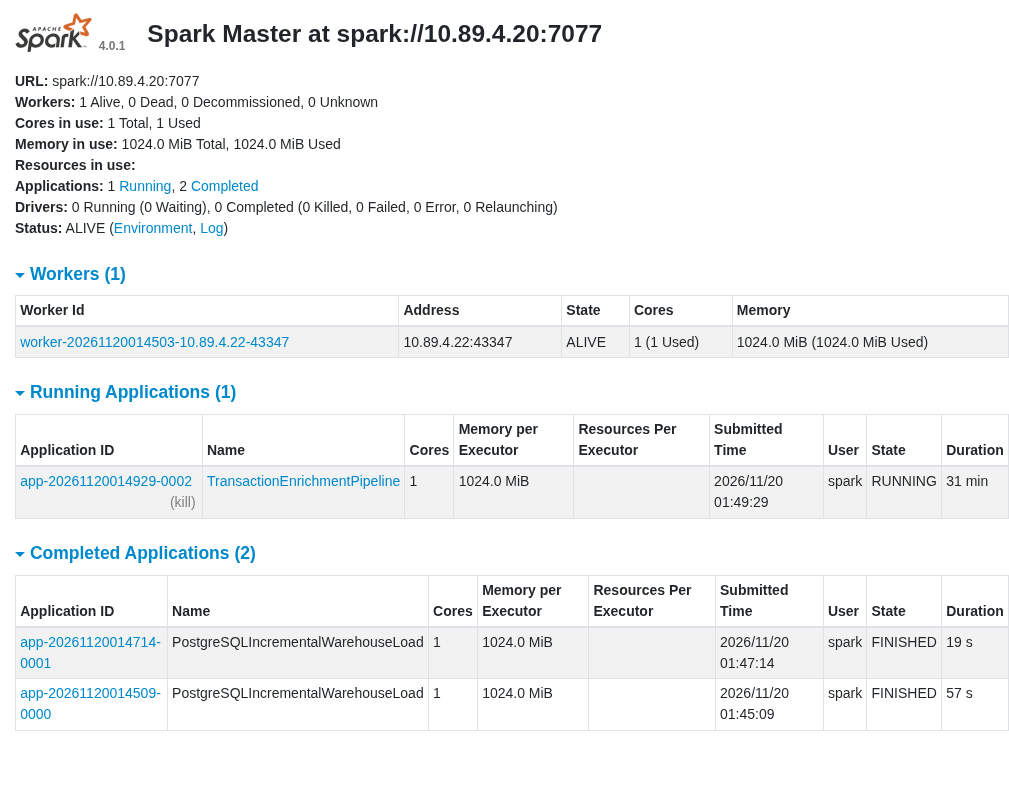
\includegraphics[width=.96\textwidth]{figures/spark_master.png}
\caption{Spark Master avec un worker actif et une application streaming en cours.}
\label{fig:sparkui}
\end{figure}

Spark Standalone alloue un cœur et 1024\,MiB au worker unique. Le traitement
batch termine ses applications dans le déploiement observé. L'application
streaming reste active sur le worker pendant la démonstration.

\chapter{Catalogue Apache Hive}

\section{Metastore et HiveServer2}
Hive utilise un Metastore autonome dont le catalogue Derby est conservé dans
un volume Podman. HiveServer2 expose Beeline sur le port 10000 et l'interface
Web sur le port 10002. Les tables sont externes : Hive conserve les
métadonnées et le schéma, tandis que les données restent dans HDFS Parquet.

\begin{figure}[H]
\centering
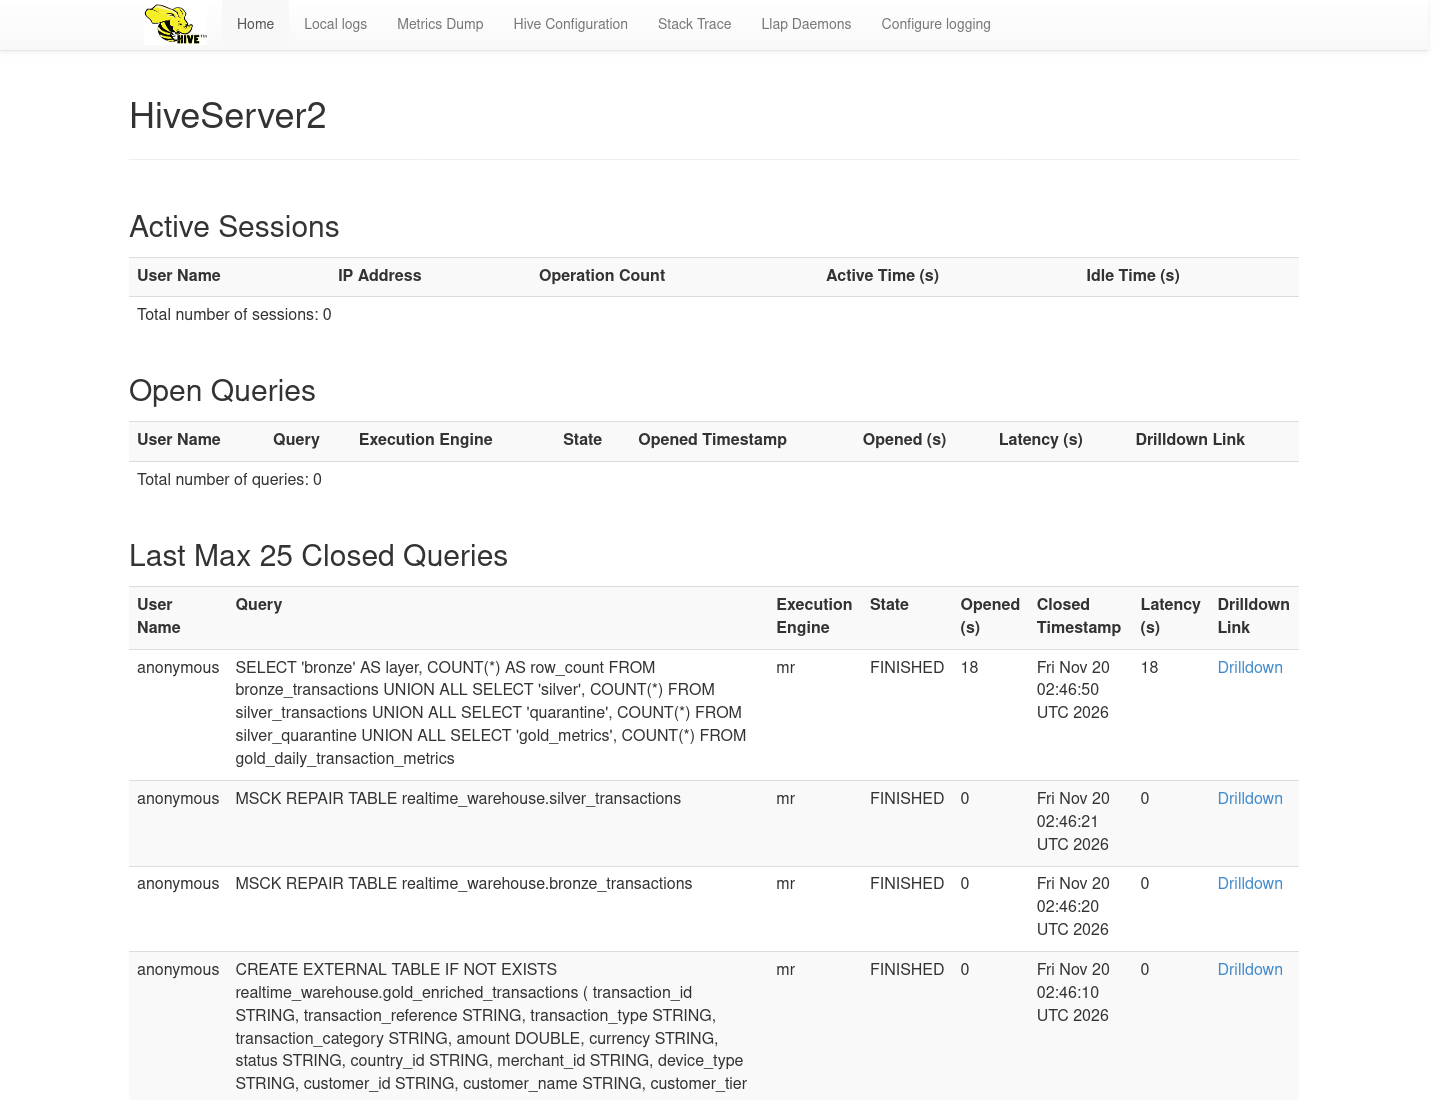
\includegraphics[width=.96\textwidth]{figures/hive_ui.png}
\caption{Interface HiveServer2 montrant les requêtes HiveQL exécutées le 20 novembre 2026.}
\label{fig:hiveui}
\end{figure}

\section{Tables externes enregistrées}
\begin{table}[H]
\centering
\begin{tabularx}{\textwidth}{Y Y}
\toprule
\textbf{Table Hive} & \textbf{Emplacement HDFS}\\
\midrule
\texttt{bronze\_transactions} & \texttt{/warehouse/bronze/transactions}\\
\texttt{silver\_transactions} & \texttt{/warehouse/silver/transactions}\\
\texttt{silver\_quarantine} & \texttt{/warehouse/silver/quarantine}\\
\texttt{gold\_daily\_transaction\_metrics} & \path{/warehouse/gold/daily_transaction_metrics}\\
\texttt{gold\_enriched\_transactions} & \texttt{/warehouse/gold/enriched\_transactions}\\
\bottomrule
\end{tabularx}
\caption{Mapping Hive/HDFS.}
\end{table}

\section{HiveQL validé}
Les requêtes suivantes ont été exécutées avec succès :
\begin{lstlisting}[language=SQL,caption={Démonstration HiveQL locale}]
SHOW TABLES;

DESCRIBE gold_daily_transaction_metrics;

SELECT * FROM gold_daily_transaction_metrics LIMIT 5;

SELECT COUNT(*) AS gold_row_count
FROM gold_daily_transaction_metrics;

SELECT currency,
       SUM(transaction_count) AS transaction_count
FROM gold_daily_transaction_metrics
GROUP BY currency
ORDER BY transaction_count DESC;
\end{lstlisting}

Le résultat du regroupement par devise confirme que Hive lit les fichiers Gold
Parquet enregistrés dans le Metastore :

\begin{table}[H]
\centering
\begin{tabular}{lr}
\toprule
\textbf{Devise} & \textbf{Transactions agrégées}\\
\midrule
EUR & 41\,993\\
AUD & 21\,193\\
INR & 21\,130\\
GBP & 21\,038\\
CAD & 21\,027\\
USD & 21\,018\\
\midrule
Total & 147\,399\\
\bottomrule
\end{tabular}
\caption{Résultat réel de la requête HiveQL \texttt{GROUP BY currency}.}
\label{tab:hiveql-result}
\end{table}

Pour ces agrégations, Hive exécute MapReduce en mode local dans le conteneur.
Le profil \texttt{full} ajoute YARN au cluster, mais la configuration Hive du
projet reste en mode local afin de limiter les dépendances et les ressources.

\chapter{Tableau de bord Streamlit}

\section{Choix de Streamlit}
Streamlit fournit l'interface de visualisation du projet et lit les indicateurs
Gold dans PostgreSQL. Le tableau de bord est disponible sur
\texttt{http://localhost:8501}.

\begin{figure}[H]
\centering
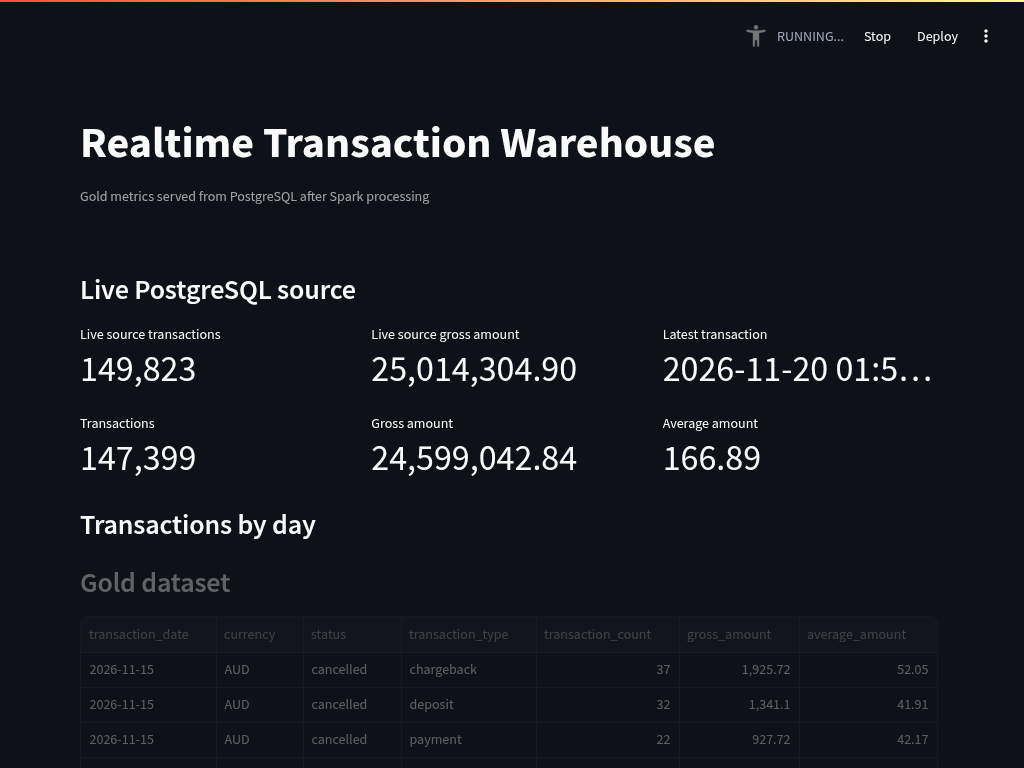
\includegraphics[width=.96\textwidth]{figures/streamlit_dashboard.png}
\caption{Tableau de bord Streamlit final.}
\label{fig:streamlit}
\end{figure}

\section{Modèle de consommation}
Streamlit lit PostgreSQL toutes les deux secondes pour afficher :
\begin{itemize}
\item le nombre de transactions sources ;
\item le montant source cumulé ;
\item l'heure de la dernière transaction ;
\item les transactions par jour ;
\item la répartition par devise ;
\item la répartition par statut ;
\item le dataset Gold détaillé.
\end{itemize}

\section{Pourquoi Streamlit lit PostgreSQL plutôt que Hive}
PostgreSQL sert de couche de diffusion rapide pour les agrégations batch.
Hive reste la couche analytique/HDFS destinée aux démonstrations HiveQL.
Cette séparation évite que le tableau de bord ait besoin d'attendre
HiveServer2 ou MapReduce pour afficher les compteurs opérationnels.

\chapter{Validation et résultats}

\section{Résultats mesurés}
\begin{table}[H]
\centering
\begin{tabularx}{\textwidth}{Y r Y}
\toprule
\textbf{Mesure (20/11/2026)} & \textbf{Valeur} & \textbf{Interprétation}\\
\midrule
Transactions PostgreSQL & 149\,823 & Source opérationnelle observée\\
Lignes Bronze lues par Hive & 147\,503 & Dernier chargement batch terminé\\
Lignes Silver lues par Hive & 147\,399 & Après déduplication et validation\\
Lignes en Quarantine & 0 & Aucune ligne invalide dans cet échantillon\\
Lignes Gold agrégées & 720 & Groupes date/devise/statut/type\\
Tables Hive & 5 & Bronze, Silver, Quarantine, Gold batch, Gold streaming\\
DataNodes vivantes & 1 & DataNode active dans le déploiement présenté\\
Workers Spark & 1 & Ressource unique suffisante pour la démonstration\\
Spark worker & 1024\,MiB & Limite configurée\\
Safe mode HDFS & OFF & Cluster opérationnel\\
\bottomrule
\end{tabularx}
\caption{Indicateurs finaux de validation observés le 20 novembre 2026.}
\end{table}

Au moment de la capture, la source PostgreSQL contenait 2\,320 lignes de plus
que le dernier lot écrit dans Bronze. Le producteur avait continué à alimenter
la source après ce lot ; le prochain chargement incrémental devait rattraper cet
écart. La différence entre Bronze et Silver (104 lignes) correspond aux
identifiants en double éliminés avant l'agrégation. Le contrôle HiveQL a aussi
confirmé zéro ligne dans Quarantine pour cet échantillon.

\section{Validation des composants}
\begin{table}[H]
\centering
\begin{tabularx}{\textwidth}{Y Y Y}
\toprule
\textbf{Composant} & \textbf{Contrôle} & \textbf{Résultat}\\
\midrule
PostgreSQL & santé + SQL & PASS\\
Kafka & topics créés & PASS\\
Spark Streaming & pipeline démarré & PASS\\
HDFS & lecture des chemins & PASS\\
Hive Metastore & santé & PASS\\
HiveServer2 & Beeline & PASS\\
HiveQL COUNT & MapReduce local & PASS\\
HiveQL GROUP BY & MapReduce local & PASS\\
Streamlit & dashboard HTTP & PASS\\
Compose & profils validés & PASS\\
Tests Python & contrats projet & PASS\\
\bottomrule
\end{tabularx}
\caption{Synthèse des validations.}
\end{table}

\section{Reproductibilité}
Le dépôt contient des commandes Make, des scripts Podman et des tests unitaires
pour vérifier la structure projet. Trois tests contractuels valident les
tables Hive, la structure des profils de déploiement et l'analyse syntaxique des sources
Python.

\chapter{Automatisation et exploitation}

\section{Commandes principales}
\begin{lstlisting}[language=bash,caption={Séquence complète de démonstration}]
cd ~/Downloads/M2/dataops/projet\ hive

make light-up
make batch
make streaming
make dashboard
make hive
make hive-demo
\end{lstlisting}

La figure~\ref{fig:terminal-startup} montre le démarrage exécuté avec
\texttt{make light-up}. Les figures~\ref{fig:terminal-postgres} et
\ref{fig:terminal-hiveql} présentent des requêtes exécutées ensuite contre
les conteneurs PostgreSQL et HiveServer2 actifs. Les valeurs correspondent
aux résultats affichés par les commandes capturées.

\begin{figure}[H]
\centering
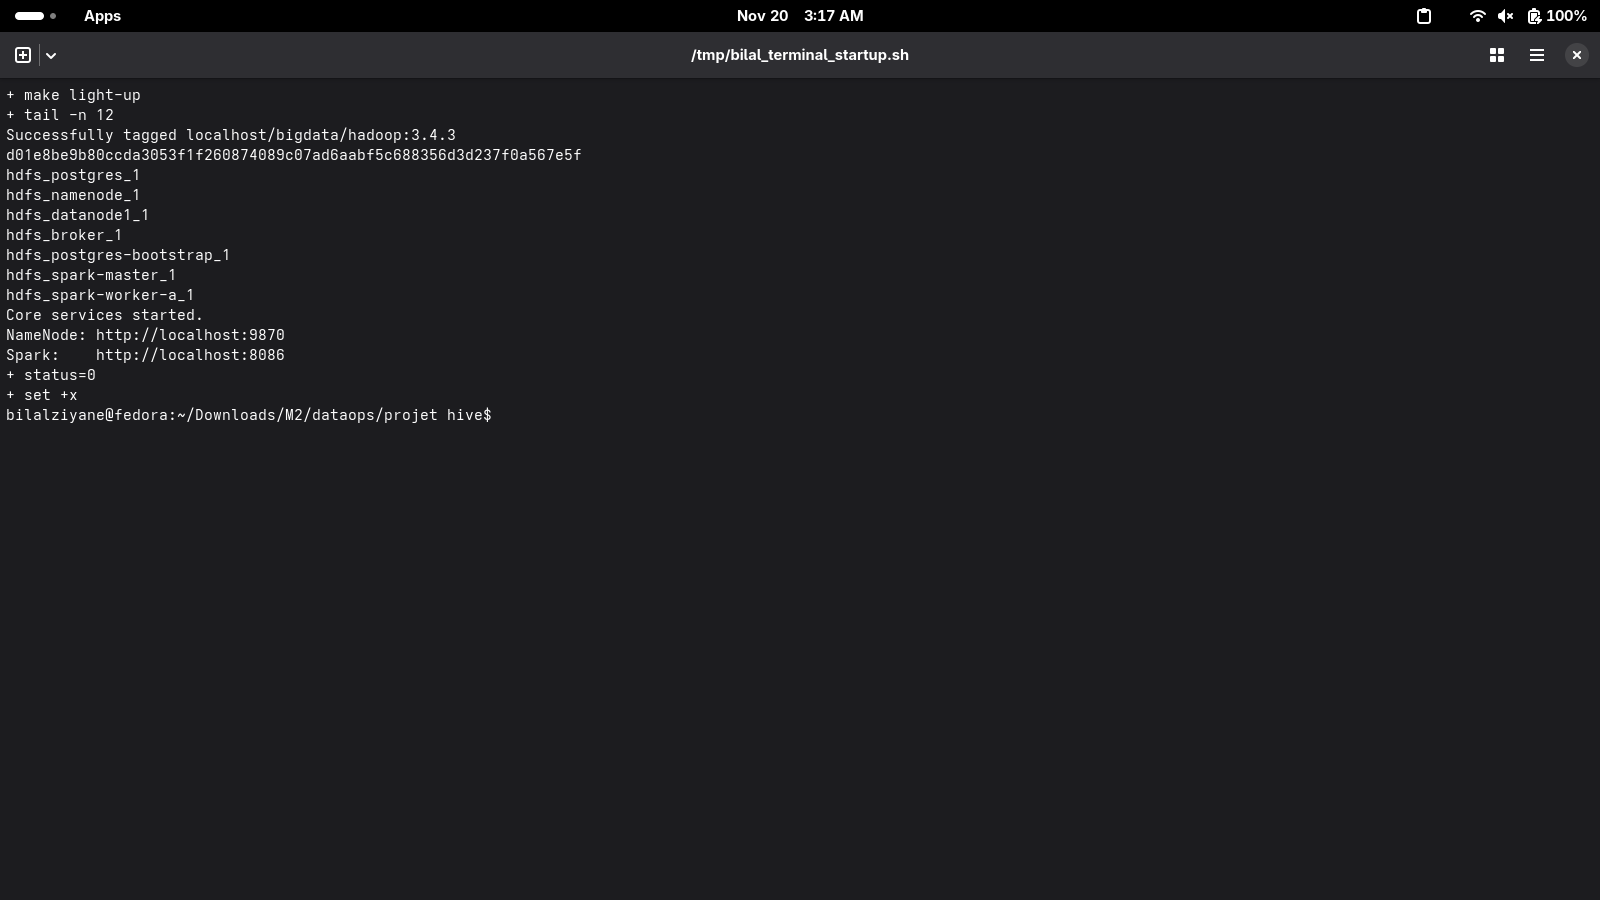
\includegraphics[width=.96\textwidth]{figures/terminal_startup.png}
\caption{Démarrage du projet avec \texttt{make light-up}.}
\label{fig:terminal-startup}
\end{figure}

\begin{figure}[H]
\centering
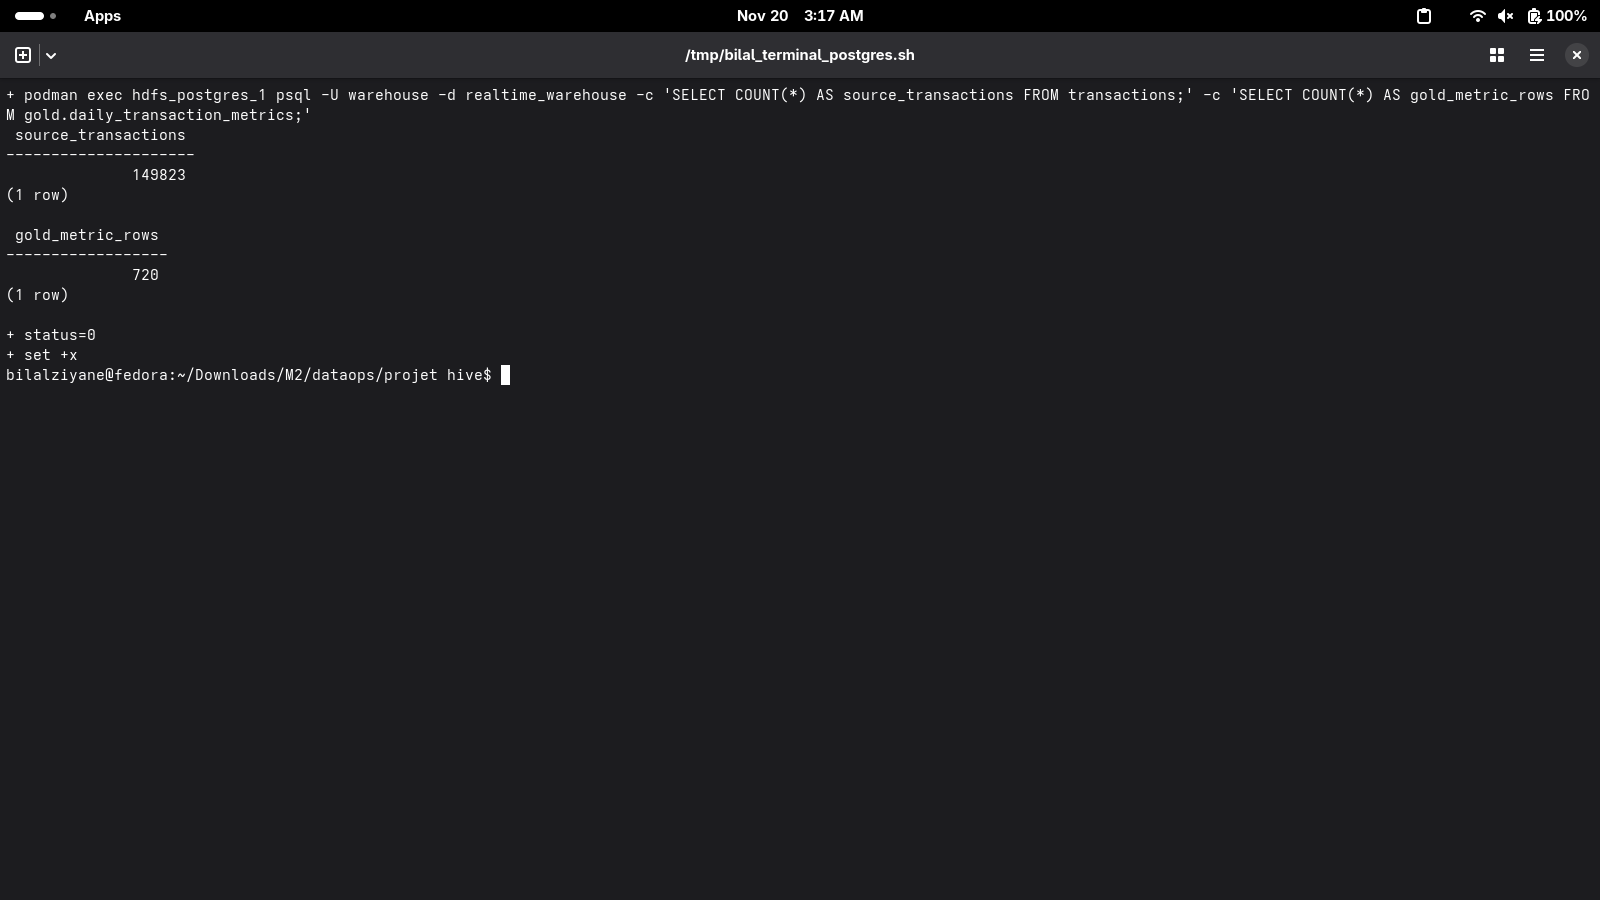
\includegraphics[width=.96\textwidth]{figures/terminal_postgresql_sql.png}
\caption{Requêtes SQL exécutées dans PostgreSQL : comptage de la source et des lignes Gold.}
\label{fig:terminal-postgres}
\end{figure}

\begin{figure}[H]
\centering
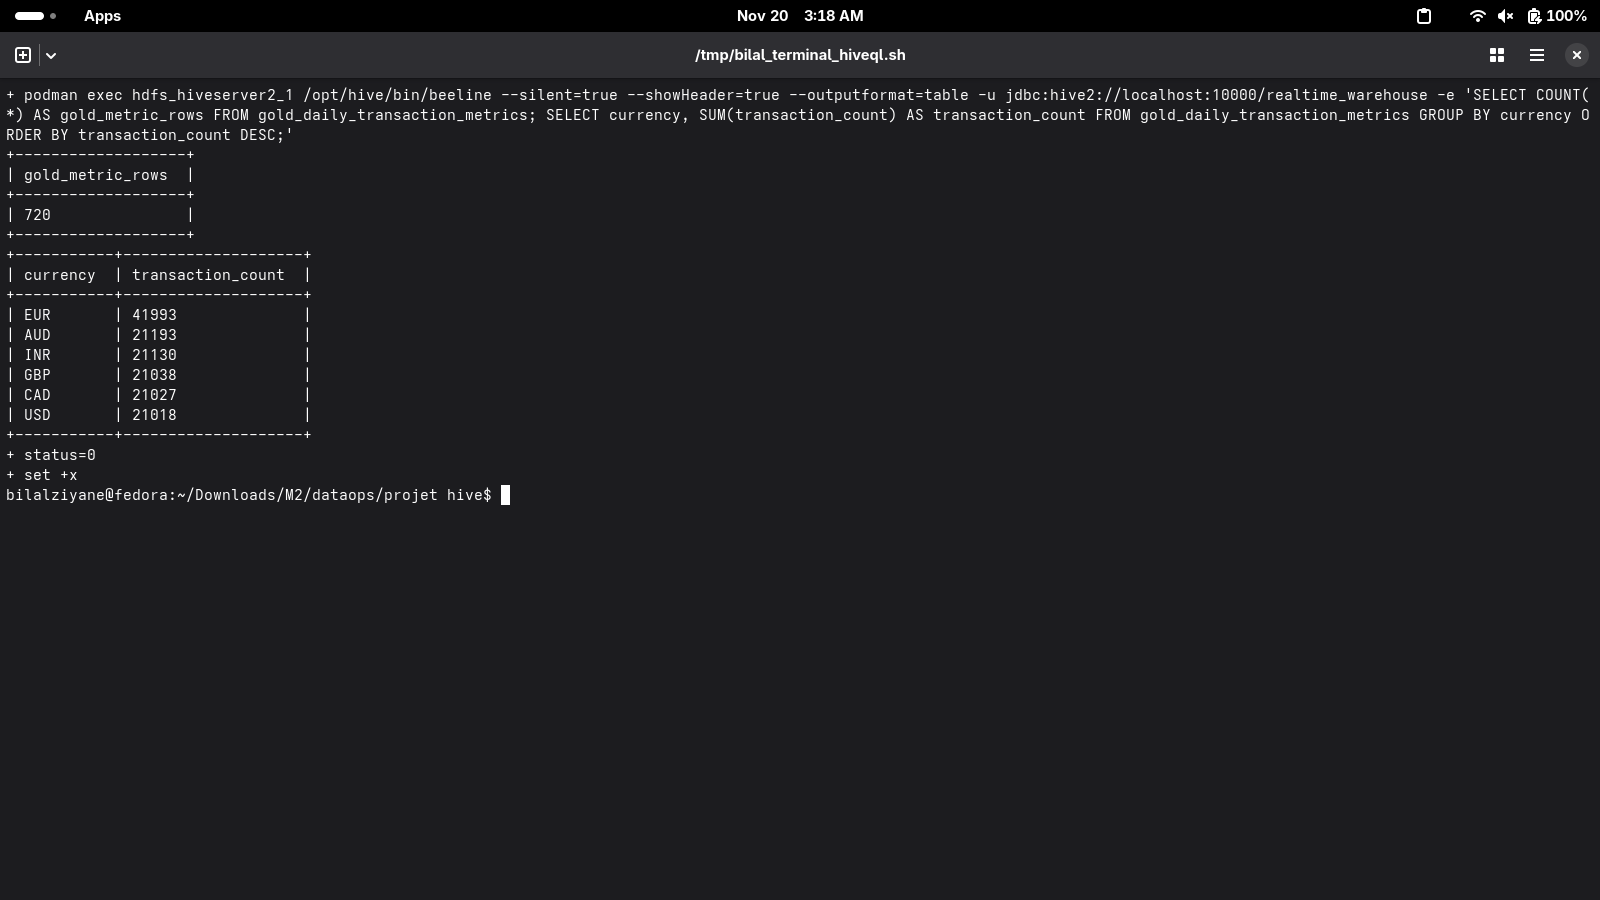
\includegraphics[width=.96\textwidth]{figures/terminal_hiveql.png}
\caption{Requêtes HiveQL exécutées dans HiveServer2 : comptage Gold et regroupement par devise.}
\label{fig:terminal-hiveql}
\end{figure}

\section{Séquence à l'oral}
\begin{enumerate}
\item Présenter l'architecture et la substitution PostgreSQL.
\item Vérifier PostgreSQL.
\item Montrer les zones Bronze, Silver, Gold et Quarantine.
\item Démarrer Kafka et Spark Streaming.
\item Expliquer les enrichissements temps réel.
\item Montrer les tables Hive et une requête GROUP BY.
\item Ouvrir Streamlit.
\item Présenter les limites de disponibilité et de parallélisme du déploiement.
\end{enumerate}

\chapter{Limites et perspectives}

\section{Limites actuelles}
\begin{itemize}
\item Une DataNode ne fournit aucune tolérance aux pannes.
\item Un seul worker Spark limite le parallélisme.
\item Le Metastore Hive utilise Derby dans le déploiement de démonstration.
\item Hive local MapReduce peut être lent pour les agrégations importantes.
\item Streamlit affiche principalement le PostgreSQL Gold, pas directement tout le catalogue Hive.
\item Les identifiants locaux sont adaptés à une démonstration de cours.
\end{itemize}

\section{Améliorations possibles}
\begin{enumerate}
\item Connecter Streamlit directement à Hive en complément de PostgreSQL.
\item Ajouter Kafka Direct-to-Hive ou Iceberg pour l'atomicité analytique.
\item Introduire dbt pour tester les transformations en médaillon.
\item Ajouter Apache Airflow pour l'orchestration batch.
\item Remplacer le Metastore Derby par PostgreSQL.
\item Ajouter observabilité Prometheus/Grafana.
\item Durcir les secrets avec Podman secrets ou Vault.
\item Ajouter CI pour les tests Compose, Python et Spark.
\end{enumerate}

\chapter{Conclusion}

La réalisation livre un pipeline cohérent entre données opérationnelles,
traitement batch, streaming, stockage HDFS, catalogue Hive et tableau de bord.
PostgreSQL remplace SQL Server conformément au choix demandé. Spark assure
les transformations batch et temps réel. Kafka relie le producteur aux
applications Streaming. HDFS conserve les couches Bronze, Silver, Gold,
Quarantine et enrichies. Hive expose les fichiers à travers un Metastore.
Streamlit offre une interface rapide adaptée à la machine disponible.

Le déploiement présenté est mono-nœud pour HDFS et Spark ; il ne fournit donc
pas de haute disponibilité et offre un parallélisme limité. Ces limites sont
compatibles avec une démonstration académique des flux batch, streaming et
HiveQL, et constituent des pistes d'évolution vers un cluster distribué.

\appendix

\chapter{Schéma technique complet}

\begin{figure}[H]
\centering
\begin{tikzpicture}[node distance=8mm,
  stage/.style={draw,rounded corners=3pt,minimum height=15mm,text width=31mm,
                align=center,fill=lightgray},
  arrow/.style={-{Stealth[length=2.5mm]},very thick}]
\node[stage,fill=blue!12] (source) {PostgreSQL\\transactions};
\node[stage,right=of source] (producer) {Producer\\Kafka};
\node[stage,right=of producer] (kafka) {Kafka\\2 topics};
\node[stage,right=of kafka] (spark) {Spark\\Batch/Streaming};
\node[stage,below=12mm of spark,fill=orange!18] (bronze) {Bronze};
\node[stage,left=of bronze,fill=gray!18] (silver) {Silver};
\node[stage,left=of silver,fill=gold!25] (gold) {Gold};
\node[stage,below=12mm of gold] (hive) {Hive\\Metastore};
\node[stage,right=of hive,fill=green!12] (dash) {Streamlit};
\draw[arrow] (producer) -- (source);
\draw[arrow] (producer) -- (kafka);
\draw[arrow] (kafka) -- (spark);
\draw[arrow] (spark) -- (bronze);
\draw[arrow] (bronze) -- (silver);
\draw[arrow] (silver) -- (gold);
\draw[arrow] (gold) -- (hive);
\draw[arrow] (source.south) |- (dash.south);
\end{tikzpicture}
\caption{Vue technique complète pour l'annexe.}
\end{figure}

\chapter{Commandes de validation finales}
\begin{lstlisting}[language=bash]
make check
make light-up
make batch
make streaming
make hive
make hive-demo
make dashboard
make stop-optional
\end{lstlisting}

\chapter{Images capturées}
Les captures du rapport proviennent du projet réel :
\begin{itemize}
\item schéma de référence ;
\item interface HDFS NameNode ;
\item interface Spark Master ;
\item interface HiveServer2 ;
\item tableau de bord Streamlit ;
\item démarrage du projet et résultats SQL/HiveQL capturés en terminal.
\end{itemize}

\begin{thebibliography}{99}
\bibitem{postgres}
PostgreSQL Global Development Group, \emph{PostgreSQL 16 Documentation}.
\url{https://www.postgresql.org/docs/16/} (consulté le 20 novembre 2026).

\bibitem{kafka}
Apache Software Foundation, \emph{Apache Kafka Documentation}.
\url{https://kafka.apache.org/documentation/} (consulté le 20 novembre 2026).

\bibitem{spark}
Apache Software Foundation, \emph{Spark Structured Streaming Programming Guide}, 4.0.1.
\url{https://spark.apache.org/docs/4.0.1/structured-streaming-programming-guide.html}
(consulté le 20 novembre 2026).

\bibitem{hadoop}
Apache Software Foundation, \emph{Hadoop Documentation}, 3.4.3.
\url{https://hadoop.apache.org/docs/r3.4.3/} (consulté le 20 novembre 2026).

\bibitem{hive}
Apache Software Foundation, \emph{Apache Hive Quickstart and HiveQL Documentation}, image 4.0.1.
\url{https://hive.apache.org/development/quickstart/} (consulté le 20 novembre 2026).

\bibitem{podman}
Podman Project, \emph{Podman Documentation}.
\url{https://docs.podman.io/} (consulté le 20 novembre 2026).

\bibitem{streamlit}
Streamlit Inc., \emph{Streamlit Documentation}.
\url{https://docs.streamlit.io/} (consulté le 20 novembre 2026).
\end{thebibliography}

\end{document}
